
\section{Definition of three major types of construtors for the SiconosmodelXML objects.}


\subsection{Default constructor}

\subsection{Constructor from an XML node}


\section{Detailed implementation of the Model Loading : Unfolding of the creation of the platform}
The two ways to construct the platform are using similar mechanisms, and especially the same creating
method.



\subsection{Model loading form an XML file}




\begin{figure}
\begin{center}
        \includegraphics[scale=0.75, clip]{figure/platform_loading_XML.ps}
        \caption{Sequence diagram of the platform's loading with XML file}
        \label{fig: platform's loading1}
\end{center}
\end{figure}

The "create"methods used are partially shown in the diagram \ref{fig: platform's loading1}.

\paragraph{Partial XML file}
This means that the data read in the file are supplemented with information given in the command
program.
In this case, the XML file is similar to the previous case, then the way to create objects of
the platform apart from a XML file will be detailed in the next section.




At first, when a XML file is loaded, the data of the file are copied in memory in a DOM tree. From
there, the XML Management platform is built.\\
The SiconosModelXML owns the DOM tree and create NSDSXML and StrategyXML objects. The created objects
only know the branch of the DOM tree relating to them. Gradually, the NSDSXML will create the
different XML objects of the dynamical systems (DSXML, LagrangianNLDSXML, LagrangianTIDSXML,
LinearSystemDSXML), and the different interactions.\\
Then, after all the XML objects have been created, the \ac{siconos} platform is built.\\
The Model which has lead the construction of the XML platform begin the creation of the NSDS,
DynamicalSystem, LagrangianNLDS, ..., Interaction, Relation, ..., NonSmoothLaw, ..., Strategy,
TimeDiscretisation, OneStepIntegrator, Moreau, ..., OneStepNSProblem, LCP and QP by using the
relating XML objects.\\
The construction of each object of the platform is made by calling a
"createXxxxx" method (createModel(...), createNSDS(...), createStrategy(...), ...). One parameter
corresponding to the XML object is enough to give the right data to the platform's object for his
construction.


\subsection{Creating model through the API}
 The unfolding of the building of the platform's architecture is described in the next sequence diagram.
\begin{figure}
\begin{center}
        \includegraphics[scale=0.75, clip]{figure/platform_loading.ps}
        \caption{Sequence diagram of the platform's loading without XML file}
        \label{fig: platform's loading2}
\end{center}
\end{figure}

The construction of the platform we can see in the diagram \ref{fig: platform's loading2} is lead by an user. And the same "createXxxxx" functions are used, like with a XML file.



Another way to build the platform is to do it manually.
To do this, each object of the \ac{siconos} platform owns functions designed to create/add the
platform's objects belonging to it. These functions must have in parameters all the required data for
the C++ objects. Here are these methods :
\begin{itemize}
        \item In the Model class :
        \begin{itemize}
                \item createNSDS(attributes required for a NSDS : bool BVP)
                \item createTimeStepping()
                \item createEvenrDriven()
        \end{itemize}
        
        \item In the NSDS class :
        \begin{itemize}
                \item addNonLinearSystemDS(number, n, x0, BasicPlugin:vectorField)
                \item addLinearSystemDS(number, n, x0)
                \item addLagrangianNLDS(number, ndof, q0, velocity0, BasicPlugin:computeMass,
                BasicPlugin:computeFInt, BasicPlugin:computeFExt,
                BasicPlugin:computeJacobianQFInt, BasicPlugin:computeJacobianVelocityFInt,
                BasicPlugin:computeJacobianQQNLInertia,
                BasicPlugin:computeJacobianVelocityQNLInertia, BasicPlugin:computeQNLInertia)
                \item addLagrangianTIDS(number, ndof, q0, velocity0, BasicPlugin:computeMass, BasicPlugin:computeFExt, K, C)
                \item addInteraction(number)
        \end{itemize}
        
        \item In the DynamicalSystem class :
        \begin{itemize}
                \item createLinearBC()
                \item createNLinearBC()
                \item createPeriodicBC()
        \end{itemize}
        
        \item In the Interaction class :
        \begin{itemize}
                \item createLagrangianLinearR()
                \item createLagrangianNonLinearR()
                \item createLinearTIR()
                \item createNewtonImpactLawNSL()
                \item createComplementaryConditionNSL()
                \item createRelayNSL()
        \end{itemize}
        
        \item In the Strategy class :
        \begin{itemize}
                \item createTimeDiscretisation()
                \item addMoreau()
                \item addLsodar()
                \item addAdams()
                \item addLCP()
                \item addQP()
        \end{itemize}
        
\end{itemize}
All these functions are calling the createXxxx(...) function of the object to create.


\section{Validation of data}


When a XML file bring the data needed by the platform, either all the data are given by the XML file or only required data. When the file contains partial data, that means it describe at least a SiconosModel with a NSDS (Non Smooth Dynamical System), composed of at least one Dynamical System.

\section{Saving the data of the platform in a XML file}
The save of the platform's data is lead from the Model. The function which do this job is
"saveToXMLFile". It has several things to do before saving tha data in a XML file :
\begin{itemize}
        \item checkXMLPlatform() : This first function will perfom verifications on the XML Management platform. It checks the
        link between the platform's objects and the XML Management objects. If the XML Management
        platform doesn't exist, it will be created and linked to the objects of the \ac{siconos}
        platform. Otherwise, every link between the platform and the XML Management is checked to ensure
        the availability of the XML platform objects.
        \item savePlatformToXML() : Now, all the objects of the platform are linked to their XML Management object. Therefore,
        it is possible to save the data of the platform to the XML DOM tree. The information
        contained in the platform are saved in the DOM tree by using the specific functions given
        by the XML object.
        \item checkXMLDOMTree() : The data of the DOM tree is up to date. But It is important to check that these data still
        respect the XML schema. 
        \item saveSiconosModelInXMLFile(xmlFile) : The last action to be done is to write the data in memory to a file.
\end{itemize}





